%% -*- coding: utf-8; -*-

% Use 'digital' option to enable back references. This option is recommended for digital pdf version
%\documentclass[phd,american,digital]{thesispuc}%english thesis
\documentclass[mscr,american]{thesispuc}%english dissertation
%\documentclass[phd,brazilian]{thesispuc}%tese em portugês
%\documentclass[msc,brazilian]{thesispuc}%disseretação em portuguŝ


%%%
%%% Additional Packages
%%%
\usepackage{tabularx}
\usepackage{multirow}
\usepackage{multicol}
\usepackage{colortbl}
\usepackage[%
    dvipsnames,
    svgnames,
    x11names,
    fixpdftex,
    table
]{xcolor}
\usepackage{numprint}
\usepackage{textcomp}
\usepackage{booktabs}
\usepackage{amsmath}
\usepackage{enumitem}
\usepackage{amssymb}
% ABNT reference style package. The current style is the alphabetical order, if you need
% change to citation order, change in the line above 'alf' to 'num', also at the end replace
% bibliographystyle with the commented version.
\usepackage[alf,bibjustif,abnt-emphasize=bf]{abntex2cite}
%\usepackage{tikz}
%\usepackage[linesnumbered, ruled, vlined]{algorithm2e}
%\usepackage{pgfplots,pgfplotstable} 
%\usepackage{array}

%% numprint 
\npthousandsep{.}
\npdecimalsign{,}

%% ThesisPUC option
%\tablesmode{fig} %% [nada, fig, tab ou figtab]
%\algoritmsmode{none} %% [none ou use] %% Default is [use]
%\codesmode{none} %% [none ou use] %% Default is [use]
%\abreviationsmode{none} %% [none ou use] %% Default is [use]

% \makeatletter  \renewcommand\@biblabel[1]{#1}  \makeatother

%%%
%%% Counters
%%%

%% uncomment and change for other depth values
\setcounter{tocdepth}{1}
%\setcounter{lofdepth}{3}
%\setcounter{lotdepth}{3}
%\setcounter{secnumdepth}{3}

%%%
%%% Misc.
%%%

\usecolour{true}


%%%
%%% Titulos
%%%

\author{Felipe V. Côrtes}
\authorR{Cortes,Felipe} % full name

\advisor{Roberto Ierusalimschy}{Prof.} %Name LastName
\advisorR{Ierusalimschy, Roberto} %LastName, Name
% If the advisor's department is different from author's department, uncomment the next line and type the correct name and acronym of advisor's institution.
%\advisorInst{institution name}{acronym}

%\coadvisor{Otávio da Fonseca Martins Gomes}{Dr.}
%\coadvisorR{da Fonseca Martins Gomes, Otávio}
%\coadvisorInst{Centro de Tecnologia Mineral}{CETEM/MCTI}

\title{Extrator de tipos} %title in portuguese

\titleuk{Type Extractor} %title in english

%%\subtitulo{Aqui vai o subtitulo caso precise}

\day{8}
\month{March}
\year{2018}

\city{Rio de Janeiro}
\CDD{004} 
\department{Informática}
\program{Informática}
\school{Pós-Graduação em Informática}
\university{Pontifícia Universidade Católica do Rio de Janeiro}
\uni{PUC-Rio }


% %%%
% %%% Jury
% %%%

% \jury{%
%   \jurymember{Alberto Barbosa Raposo}{Prof.}
%     {Departamento de Informática}{PUC-Rio}
%   \jurymember{Waldemar Celes Filho}{Prof.}
%     {Departamento de Informática}{PUC-Rio}
% }


% %%%
% %%% Personal Resume
% %%%

% \resume{%
% % If it fit in one line use this command:
% \makebox[\textwidth][s]{Graduated in computer science by the  Harvard University.}%
% % If not just type your resume without any special command 
% }

% %%%
% %%% Acknowledgment (REMINDER TO SCHOLARSHIP STUDENTS. Do not forget to thank the agencies that supported your work.)
% %%%
% \acknowledgment{%
% \noindent To my adviser Professor Marcelo Gattass for the stimulus and partnership
% to carry out this work.
% \bigskip

% \noindent To CNPq and PUC-Rio, for the aids granted, without which this work does not
% could have been accomplished.
% \bigskip

% \noindent \textbf{For students contemplated with any CAPES scholarship, whose defense occurred as of 04 September 2018 leave the following passage:} 

% \noindent This study was financed in part by the Coordenação de Aperfeiçoamento de Pessoal
% de Nível Superior - Brasil (CAPES) - Finance Code 001.
% }


%%%
%%% Catalog prekeywords
%%%

\catalogprekeywords{%
  \catalogprekey{Informática}%
}

%%%
%%% Keywords - Don't use % at the end of /key dfinition
%%%

\keywords{%
  \key{Procesamento Geométrico}
  \key{Remoção de ruído de malha}
  \key{Vizinhança adaptativa}
}

\keywordsuk{%
  \key{Geometry Processing}
  \key{Mesh Denoising}
  \key{Adaptive Patches}
}

%%%
%%% Abstract
%%%

% \abstract{%
% A aquisição de malhas triangulares normalmente introduz ruídos indesejados...
% }

% \abstractuk{%
% The acquisition of triangular meshes typically introduces undesired noise...}

%%%
%%% Dedication
%%%

\dedication{%
  To my parents, for their support\\
and encouragement.
}

%%%
%%% Epigraph
%%%

% \epigraph{%
%   My beautifull epigraph
% }
% \epigraphauthor{Wassily Kandinsky}
% \epigraphbook{Regards sur le passé}


\begin{document}
  % -*- coding: utf-8; -*-

\chapter{Introduction}
There are several reasons that motivate the adoption of statically typed languages. Maintaining large systems built with dynamic types can become a nightmare due to the lack of type information \cite{takikawa_is_2016}. Typed languages also generally has better performance because compile-time type information helps generating optimized machine code. However, programmers are frequently left empty-handed when inspecting dynamically typed code while having to re-write systems to a statically typed languaged if gradually typed languages are not an option.
\paragraph*{}
Inspired by the challenge of inspecting dynamically typed code, we built a type extractor for the Lua programming language. By inspecting a program's execution during runtime, it can generate enough information to help programmers visualize the types being transfered between functions of their program. The software output can be used as an useful documentation, while also helping programmers migrate code to a statically typed one or even for debugging.
\paragraph*{}
The document is structured as follows. In Chapter ~\ref{cha:Previous Work} we present previous work related to type systems in Lua. In Chapter ~\ref{cha:Project Scope} we describe the software goal. Chapter ~\ref{cha:Project Specification} explain the software modules and how they interact. In Chapter ~\ref{cha:Development} it's shown the software key functions, the modules relationship and basic utilization. In Chapter ~\ref{cha:Results} we present and discuss some results obtained by the type extractor on some Lua benchmarks. Finally on Chapter ~\ref{cha:Final Considerations} we present our conclusion and future work.

% \begin{figure}
% \centering
% 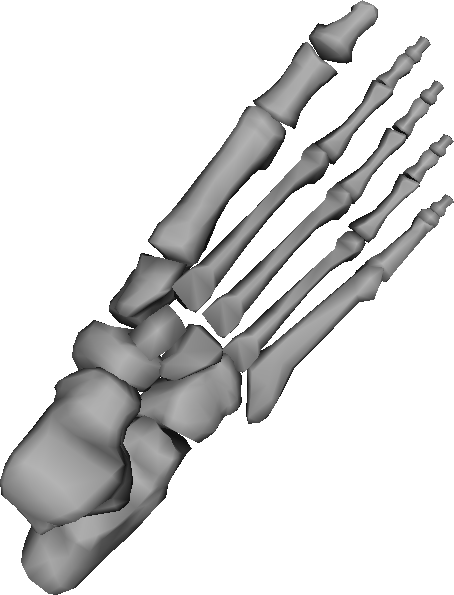
\includegraphics[width=0.45\textwidth]{pictures/image01.png}
% 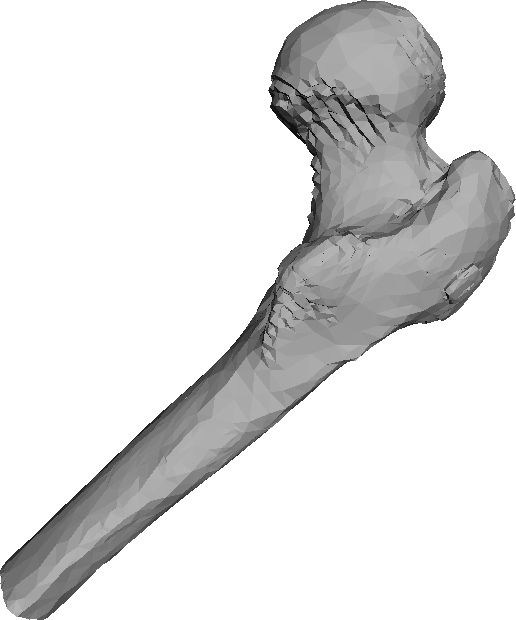
\includegraphics[width=0.45\textwidth]{pictures/image02.png}
% \caption{Meshes generated from medical data. Data obtained from the AIM$@$SHAPE Shape Repository \cite{AIMSHAPE}}
% \label{fig:example}
% \end{figure}

%This document is structured as follows. In Chapter~\ref{cha:Previous Work} we present some previous work relevant to our problem. In Chapter~\ref{cha:Proposal} we explain our proposal. In Chapter~\ref{cha:Results} we show our results. Finally, in Chapter~\ref{cha:Conclusion} we present our conclusion and future work.


 % introduction
  % -*- coding: utf-8; -*-

\chapter{Project Scope}
The extractor can analyse each function call and return by using reflection properties of the Lua programming language. With the debug library, we ca\
n register hook functions to inspect the behaviour of a program's execution and then compute the types of functions and variables present in the code\
.
\newline
The Type Extractor can be used by two approaches.
\begin{itemize}
    \item{Full Analysis:} A full program analysis can be made by passing a Lua program as input to the extractor. In this approach, each possible fun\
ction call and return types will be analysed.
    \item{Inspection library:} An auxiliar library, capable of registring specific functions for inspection. In this approach, the programmer can sel\
ect what part of the program they want to analyse.
\end{itemize}
In the end of each execution, a report will be generated. This report has information about parameters and return types of each analysed function.
\newline
These usage scenarios enables the extractor to be used as an auxiliary tool for migrating from dynamically to statically typed languages. It also ser\
ves as a good documentation for functions parameter and return types. Giving tools for understanding the type relations inside a program helps progra\
mmers to debug and optimize dynamically typed code.

%This document is structured as follows. In Chapter~\ref{cha:Previous Work} we present some previous work relevant to our problem. In Chapter~\ref{cha:Proposal} we explain our proposal. In Chapter~\ref{cha:Results} we show our results. Finally, in Chapter~\ref{cha:Conclusion} we present our conclusion and future work.


 % previous work
  % -*- coding: utf-8; -*-
\chapter{Proposal}
\label{cha:Proposal}

Equation example 1:

\begin{equation}
\begin{split}
\min_u \int_{x_i\in X}\int_{x_j\in X} q_{ij} u_i u_j da da + \int_{x_i\in X}||x' - x_i|| u_i da \\
s.t. \ \ \ u\in[0,1] \ \ \land  \ \ \int_{x_i\in X}u da = a_0,
\end{split}
\end{equation}

Equation exmaple 2:

\begin{equation}
\begin{split}
\min_{\mathbf{u}} \alpha \mathbf{u}^T \mathbf{A}^T \mathbf{Q} \mathbf{A} \mathbf{u} +  \beta \mathbf{d}^T a' \mathbf{A} \mathbf{u} + \gamma \mathbf{u}^T \mathbf{G}^T \mathbf{G} \mathbf{u} + \delta\mathbf{f}^T a' \mathbf{A} \mathbf{u} \\
s.t. \ \ \ \mathbf{0} \leq \mathbf{u} \leq \mathbf{1} \land \mathbf{a}^T\mathbf{u}=a_0.
\end{split}
\end{equation}

Equation example 3:
\begin{align}
\mathbf{G}=(g_{ij}) = \left\lbrace
\begin{array}{ll}
\sum_{f_k\in N_f(f_i)} l_{ik} & i=j\\
-l_{ij} & e_{ij}\in E\\
0 & \text{otherwise}
\end{array}
\right.
\end{align}

\lstinputlisting[label=mean,title={Mean Filter},caption={Mean Filter},language=R]{codes/mean.R}

%% Poruguese algorithm
%\begin{algorithm}
%\DontPrintSemicolon
%\Entrada{Malha e quantidade de pontos a ser amostrado}
%\Saida{Pontos amostrados na malha}
%\BlankLine
%\emph{Crie um vetor de números randômicos entre $[0,1]$ com a %quantidade de pontos a ser amostrada e ordene-o}\;
%\emph{Calcule a área total dos triângulos da malha}\;
%\For{$i=0$ \KwTo numeroDePontos} {
%  \emph{Navegue entre as faces acumulando a sua $\frac{area}{areaTotal}$ até achar a face com valor acumulado $\geqslant$ numerosRandomicos[i]}\;
%  \emph{Pegue um ponto randômico dentro da face utilizando o %método de Turk e adicione no vetor do resultado}\;
%}
%\caption{Escolha das amostras inicias}\label{alg:sampling}
%\end{algorithm}\DecMargin{1em}

%% enlgish algorithm
\begin{algorithm}
\DontPrintSemicolon
\KwIn{Malha e quantidade de pontos a ser amostrado}
\KwOut{Pontos amostrados na malha}
\BlankLine
\emph{Crie um vetor de números randômicos entre $[0,1]$ com a quantidade de pontos a ser amostrada e ordene-o}\;
\emph{Calcule a área total dos triângulos da malha}\;
\For{$i=0$ \KwTo numeroDePontos} {
  \emph{Navegue entre as faces acumulando a sua $\frac{area}{areaTotal}$ até achar a face com valor acumulado $\geqslant$ numerosRandomicos[i]}\;
  \emph{Pegue um ponto randômico dentro da face utilizando o método de Turk e adicione no vetor do resultado}\;
}
\caption{Escolha das amostras inicias}\label{alg:sampling}
\end{algorithm}\DecMargin{1em}







  % -*- coding: utf-8; -*-

\chapter{Results}
\label{cha:Results}

Table example. Table~\ref{tab:res} shows results. 

\begin{table}[!h]
\caption{Results for devil mesh}
\tiny
\begin{center}
\begin{tabular}{ m{1.1cm} m{0.95cm} m{0.95cm} m{0.95cm} m{0.95cm} m{0.95cm} m{0.95cm} m{0.95cm} m{0.95cm} m{0.95cm} } 
 & Mean Vertex Distance & L2 Vertex Based & Mean Quadric & MSAE & L2 Normal Based & Tangential & Mean Discrete Curvature & Area Error & Volume Error\\ 
 \hline 
\cite{FDC03} & 0.061277 & 0.110973 & 0.236219 & 19.697900 & 0.055170 & 0.047678 & 0.090284 & 0.051443 & 0.045645 \\ 
 \cite{JDD03} & 0.001293 & 0.002800 & 0.002289 & 21.237300 & 0.021589 & 0.013026 & 0.087991 & 0.000364 & 0.002621 \\ 
 \cite{SRML07} & 0.001439 & 0.002880 & 0.003540 & 14.043200 & 0.012654 & 0.008911 & 0.055849 & 0.007806 & 0.000582 \\ 
 \cite{ZFAT11} & \cellcolor{blue!25}0.000713 & \cellcolor{blue!25}0.001537 & 0.001824 & 12.171400 & \cellcolor{blue!25}0.009654 & \cellcolor{blue!25}0.005781 & \cellcolor{blue!25}0.054567 & 0.005617 & \cellcolor{blue!25}0.000425 \\ 
 \cite{HS13} & 0.002531 & 0.004560 & 0.007108 & 13.830100 & 0.017459 & 0.010314 & 0.114528 & 0.001686 & 0.001786 \\ 
 \cite{ZDZBL15} & 0.001623 & 0.003079 & 0.005048 & \cellcolor{blue!25}10.454200 & 0.015233 & 0.008054 & 0.094668 & 0.002629 & 0.001326 \\ 
 \cite{YRP16} & 0.000737 & 0.001548 & \cellcolor{blue!25}0.001493 & 16.880800 & 0.014129 & 0.006974 & 0.079952 & \cellcolor{blue!25}0.000209 & 0.002375 \\ 
 Ours & 0.000987 & 0.001902 & 0.002686 & 11.574200 & 0.010632 & 0.006796 & 0.075106 & 0.003970 & 0.000722 \\ 
 \end{tabular}
\end{center}
 \label{tab:res}
\end{table}

\section{Comparison}
  \chapter{Conclusion and future work}
\label{cha:Conclusion}

We proposed an algorithm for triangular mesh denoising with detail preservation...

\lstinputlisting[label=mean2,title={Mean Filter},caption={Mean Filter},language=R]{codes/mean.R}
  %% ...
  \arial
  \bibliographystyle{abnt-alf} % \bibliographystyle{abnt-num}
  \bibliography{srs} 
\end{document}
